% \def\year{2022}\relax
% \def\year{2025}\relax
%File: formatting-instructions-latex-2022.tex
%release 2022.1
% \documentclass[letterpaper]{article}
% \usepackage{aaai}
% \usepackage{times}
% \usepackage{helvet}
% \usepackage{courier}
\documentclass[letterpaper]{article} % DO NOT CHANGE THIS
\usepackage[submission]{aaai2026}  % DO NOT CHANGE THIS
% \usepackage[submission]{aaai24}  % DO NOT CHANGE THIS
\usepackage{times}  % DO NOT CHANGE THIS
\usepackage{helvet}  % DO NOT CHANGE THIS
\usepackage{courier}  % DO NOT CHANGE THIS
\usepackage[hyphens]{url}  % DO NOT CHANGE THIS
\usepackage{graphicx} % DO NOT CHANGE THIS
\urlstyle{rm} % DO NOT CHANGE THIS
\def\UrlFont{\rm}  % DO NOT CHANGE THIS
\usepackage{natbib}  % DO NOT CHANGE THIS AND DO NOT ADD ANY OPTIONS TO IT
\usepackage{caption} % DO NOT CHANGE THIS AND DO NOT ADD ANY OPTIONS TO IT
\DeclareCaptionStyle{ruled}{labelfont=normalfont,labelsep=colon,strut=off} % DO NOT CHANGE THIS
\frenchspacing  % DO NOT CHANGE THIS
\setlength{\pdfpagewidth}{8.5in}  % DO NOT CHANGE THIS
\setlength{\pdfpageheight}{11in}  % DO NOT CHANGE THIS
%
% These are recommended to typeset algorithms but not required. See the subsubsection on algorithms. Remove them if you don't have algorithms in your paper.
\usepackage{algorithm}
\usepackage{algorithmic}
%-----ACM-Approved-----
% \usepackage{balance,bm}
\usepackage{color, colortbl}
\usepackage[table]{xcolor}
\usepackage{url}
% \usepackage{hyperref}
% \hypersetup{
%     colorlinks=false,
% }
\usepackage{subcaption}
\usepackage{textcomp}
\usepackage{soul}
\usepackage{multirow}
% \usepackage{wrapfig}
\usepackage{enumitem}
\usepackage{mathtools}
\usepackage{siunitx}
%---------------------

% \usepackage{subcaption}
\usepackage{booktabs} % For formal tables | Already in ACM
% \usepackage[ruled]{algorithm2e} % For algorithms
% \usepackage{graphicx} % Already in ACM
% \usepackage{url}
% \usepackage{graphicx}  %Already in ACM
\usepackage{longtable,booktabs}


%presently not allowed
% \usepackage{capt-of}
\frenchspacing  %Required

\captionsetup{compatibility=false}

% \usepackage{amsmath} %Already in ACM
% \usepackage{array} %Already in ACM
\usepackage{arydshln}
\setlength\dashlinedash{0.2pt}
\setlength\dashlinegap{1.5pt}
\setlength\arrayrulewidth{0.3pt}
% \usepackage{tcolorbox}

% \usepackage [english]{babel}
% \usepackage{url}
% \usepackage [autostyle, english = american]{csquotes}
\definecolor{linkColor}{RGB}{6,125,233}
\definecolor{green}{rgb}{0.0, 0.65, 0.31}
\definecolor{bleudefrance}{rgb}{0.19, 0.55, 0.91}
\definecolor{ceruleanblue}{rgb}{0.16, 0.32, 0.75}
\definecolor{grey}{HTML}{969696}
\definecolor{violet}{HTML}{756bb1}
\definecolor{dgrey}{HTML}{01665e}
\definecolor{lgrey}{HTML}{5ab4ac}
\definecolor{dgreen}{HTML}{005a32}
\definecolor{purple}{HTML}{ae017e}

%pt, bp, dd, mm, cm, ex, em, pc, in
\def\greybar#1{{\color{grey}\rule{#1pc}{6pt}}}
\def\dgreybar#1{{\color{dgrey}\rule{#1pc}{6pt}}}
\def\lgreybar#1{{\color{lgrey}\rule{#1pc}{6pt}}}
% \definecolor{editCol}{rgb}{0.0, 0.3, 0.5}
% \definecolor{editCol}{rgb}{0.1, 0.1, 0.8}
% \definecolor{editCol}{HTML}{0000FF}
\definecolor{editCol}{HTML}{000000}
\definecolor{maskCol}{HTML}{c51b7d}
\definecolor{lrColor}{HTML}{8856a7}
\definecolor{trColor}{HTML}{d01c8b}
\definecolor{ctColor}{HTML}{4dac26}
\definecolor{brickred}{HTML}{f03b20}

% Define colorblind-friendly significance colors (blue sequential palette)
\definecolor{sigone}{RGB}{222, 235, 247}    % p < 0.05 (lightest)
\definecolor{sigtwo}{RGB}{158, 202, 225}    % p < 0.01 (medium)
\definecolor{sigthree}{RGB}{107, 174, 214}  % p < 0.001 (darkest)

% \definecolor{sigone}{HTML}{feebe2}    % p < 0.05 (lightest)
% \definecolor{sigtwo}{HTML}{fbb4b9}    % p < 0.01 (medium)
% \definecolor{sigthree}{HTML}{f768a1}  % p < 0.001 (darkest)

% \definecolor{sigone}{HTML}{ffffff}    % p < 0.05 (lightest)
% \definecolor{sigtwo}{HTML}{ffffff}    % p < 0.01 (medium)
% \definecolor{sigthree}{HTML}{ffffff}  % p < 0.001 (darkest)

% \definecolor{improveCol}{HTML}{253494}
% \definecolor{worsenCol}{HTML}{d7191c}

\definecolor{improveCol}{HTML}{4dac26}
\definecolor{worsenCol}{HTML}{d01c8b}

% \definecolor{improveCol}{HTML}{5e3c99}
% \definecolor{worsenCol}{HTML}{e66101}
\definecolor{DarkBlue}{HTML}{00008B}
\definecolor{mscolor}{HTML}{01665e}
\definecolor{nmscolor}{HTML}{bf812d}
\definecolor{lgreen}{HTML}{ccece6}
\definecolor{dolive}{HTML}{308014}

\colorlet{tablerowcolor4}{gray!50} % Table row separator colour = 

\def\impbar#1{%%
  {\color{improveCol}\rule{#1mm}{5pt}}
  }
\def\worbar#1{%%
  {\color{worsenCol}\rule{#1mm}{5pt}}
  }
  
\def\trbar#1{%%
  {\color{trColor}\rule{#19mm}{5pt}}
  }
\def\mybar#1{%%
  {\color{bleudefrance}\rule{#19mm}{5pt}}
  }
\def\nubarGreen#1{%%
  {\color{neutralGreen}\rule{#19mm}{5pt}}
  }
 \def\nubar#1{%%
  {\color{neutralCol}\rule{#19mm}{5pt}}
  }
\def\BfBar#1{%%
  {\color{BfTrColor}\rule{#19mm}{5pt}}
  } 
  \def\AfBar#1{%%
  {\color{AfTrColor}\rule{#19mm}{5pt}}
  }
 \def\ftbar#1{%%
  {\color{tablerowcolor4}\rule{#19mm}{5pt}}
  }
  
% \def\incbar#1{%%
%   {\color{worsenCol}\rule{#19dd}{5pt}}
%   }
% \def\decbar#1{%%
%   {\color{improveCol}\rule{#19dd}{5pt}}
%   }
  
\def\incbar#1{%%
  {\color{improveCol}\rule{#19dd}{5pt}}
  }
\def\decbar#1{%%
  {\color{worsenCol}\rule{#19dd}{5pt}}
  }

  
\newcommand*{\textlabel}[2]{%
  \edef\@currentlabel{#1}% Set target label
  \phantomsection% Correct hyper reference link
  #1\label{#2}% Print and store label
}

 \newcommand{\ra}[1]{\renewcommand{\arraystretch}{#1}}
\colorlet{tableheadcolor}{gray!25} % Table header colour = 25% gray
\newcommand{\headcol}{\rowcolor{tableheadcolor}} %
\colorlet{tablerowcolor}{gray!10} % Table row separator colour = 
\colorlet{tablerowcolor2}{gray!45} % Table row separator colour = 
\colorlet{tablerowcolor3}{gray!12} % Table row separator colour = 10% gray

\newcommand{\rowcol}{\rowcolor{tablerowcolor}} %
\newcommand{\rowcolmedium}{\rowcolor{tablerowcolor2}}
\newcommand{\rowcollight}{\rowcolor{tablerowcolor3}} %

\newcommand{\mc}[2]{\multicolumn{#1}{c}{#2}}
\newcolumntype{a}{>{\columncolor{tablerowcolor}}r}
% \newcolumntype{b}{>{\columncolor{white}}c}
\definecolor{aicolor}{HTML}{018571}
\definecolor{occolor}{HTML}{ff7799}

% \definecolor{aicolor}{HTML}{018571}
% \definecolor{occolor}{HTML}{ff7799}
\definecolor{aicolor}{HTML}{fc8d62}
\definecolor{occolor}{HTML}{253494}

 \def\nuLRbar#1{%%
  {\color{dpink}\rule{#10mm}{4pt}}
  }
\def\ftbar#1{%%
  {\color{deepgrey}\rule{#1in}{6pt}}
  }

\def\aibar#1{%%
  {\color{aicolor}\rule{#11ex}{6pt}}
  }
  
\def\ocbar#1{%%
  {\color{occolor}\rule{#11ex}{6pt}}
  }

% \def\aibarr#1{%%
%   {\color{aicolor}\rule{#1cm}{6pt}}
%   }
  
% \def\ocbarr#1{%%
%   {\color{occolor}\rule{#1cm}{6pt}}
%   }

\def\aibarr#1{%%
  {\color{aicolor}\rule{#1mm}{6pt}}
  }
  
\def\ocbarr#1{%%
  {\color{occolor}\rule{#1mm}{6pt}}
  }

\newcommand{\hlAI}[1]{\colorbox{aicolor!50}{~#1}}
\newcommand{\hlOC}[1]{\colorbox{occolor!50}{#1}}
\newcommand{\edit}[1]{{\textcolor{editCol}{#1}}}
\newcommand{\mask}[1]{{\textcolor{maskCol}{#1}}}

\def\nuLRbar#1{%%
  {\color{lrColor}\rule{#10mm}{4pt}}
  }
\newcommand{\Bf}{\textit{Before}}
\newcommand{\Af}{\textit{After}}
\newcommand{\Tr}{\textit{Treated}}
\newcommand{\Ct}{\textit{Control}}

\newcommand{\bsky}{\textit{Bluesky}}
\newcommand{\news}{\texttt{News}}

\newcommand{\Is}{\textit{Isolation}}
\newcommand{\Nm}{\textit{Normalization}}
\newcommand{\Vc}{\textit{Vaccination}}

% \newcommand{\Is}{\textit{Is}}
% \newcommand{\Nm}{\textit{Nm}}
% \newcommand{\Vc}{\textit{Vc}}

\newcommand{\M}{$S_M$}
\newcommand{\Sn}{$S_1$}
\newcommand{\Snn}{$S_2$}
\newcommand{\Snnn}{$S_3$}
\newcommand{\RTE}{\textsf{RTE}}
\newcommand{\ITE}{\textsf{ITE}}
\newcommand{\ea}{\textit{et al.}}
% \newcommand{\imp}[1]{{\textcolor{improveCol}{\it#1}}}
% \newcommand{\wor}[1]{{\textcolor{worsenCol}{\it#1}}}
\newcommand{\imp}[1]{{\textcolor{improveCol}{\it#1}}}
\newcommand{\wor}[1]{{\textcolor{worsenCol}{\it#1}}}

\renewcommand{\textrightarrow}{$\rightarrow$}
\renewcommand{\textleftarrow}{$\leftarrow$}

\newcommand{\cdib}{$\mathbf{CDI}$}
% \newcommand{\somra}{$\mathnormal{LibRA}$}
\newcommand{\cdi}{$\mathtt{CDI}$}

\newcommand{\cze}{$\mathtt{C_0}$}
% \newcommand{\con}{$\mathtt{C_1}$}
\newcommand{\cone}{$\mathtt{C_1}$}
\newcommand{\ctw}{$\mathtt{C_2}$}
\newcommand{\cth}{$\mathtt{C_3}$}
\newcommand{\cfo}{$\mathtt{C_4}$}

\newcommand{\tabitem}{\textbullet~~}

% \newcommand{\ra}[1]{\renewcommand{\arraystretch}{#1}}
\colorlet{tableheadcolor}{gray!25} % Table header colour = 25% gray
% \newcommand{\headcol}{\rowcolor{tableheadcolor}} %
% \newcommand{\rowcol}{\rowcolor{tablerowcolor}} %

\definecolor{neutralCol}{HTML}{dd1c77}
\definecolor{neutralGreen}{HTML}{31a354}
\definecolor{NewBlue}{HTML}{1879ba}
\definecolor{bleudefrance}{rgb}{0.19, 0.55, 0.91}  
\definecolor{AfTrColor}{HTML}{0868ac}  
\definecolor{BfTrColor}{HTML}{a8ddb5}  

\definecolor{AfCtColor}{HTML}{b10026}  
\definecolor{BfCtColor}{HTML}{fd8d3c}

\graphicspath{ {figures/} }

% \renewcommand{\sectionautorefname}{Section}
% \renewcommand{\subsectionautorefname}{Section}
% \renewcommand{\subsubsectionautorefname}{Section}
% % \renewcommand{\subsubsectionautorefname}{Section}
% % \renewcommand{\figureautorefname}{Figure}
% \renewcommand{\figureautorefname}{Figure}

% \newcommand{\para}[1]{\vspace{1em}\noindent\textbf{#1}~}
% \newcommand{\itpara}[1]{\vspace{1em}\noindent\textit{#1}~}

\newcommand{\para}[1]{\vspace{0.2em}\noindent\textbf{\textit{#1}~}}
\newcommand{\itpara}[1]{\vspace{0.2em}\noindent\textit{#1}~}


\usepackage{xcolor}
\newcommand{\answerYes}[1]{\textcolor{blue}{#1}} 
\newcommand{\answerNo}[1]{\textcolor{teal}{#1}} 
\newcommand{\answerNA}[1]{\textcolor{gray}{#1}} 
\newcommand{\answerTODO}[1]{\textcolor{red}{#1}} 

%
% These are are recommended to typeset listings but not required. See the subsubsection on listing. Remove this block if you don't have listings in your paper.
\usepackage{newfloat}
\usepackage{listings}
\lstset{%
	basicstyle={\footnotesize\ttfamily},% footnotesize acceptable for monospace
	numbers=left,numberstyle=\footnotesize,xleftmargin=2em,% show line numbers, remove this entire line if you don't want the numbers.
	aboveskip=0pt,belowskip=0pt,%
	showstringspaces=false,tabsize=2,breaklines=true}
\floatstyle{ruled}
\newfloat{listing}{tb}{lst}{}
\floatname{listing}{Listing}
%
%\nocopyright
%
% PDF Info Is REQUIRED.
% For /Title, write your title in Mixed Case.
% Don't use accents or commands. Retain the parentheses.
% For /Author, add all authors within the parentheses,
% separated by commas. No accents, special characters
% or commands are allowed.
% Keep the /TemplateVersion tag as is
\pdfinfo{
/Title (From Web(logs) to Web(AI): Questions, Platforms, and Methods across Twenty Editions of ICWSM)
/Author ()
/TemplateVersion (2026.1)
}

% DISALLOWED PACKAGES
% \usepackage{authblk} -- This package is specifically forbidden
% \usepackage{balance} -- This package is specifically forbidden
% \usepackage{color (if used in text)
% \usepackage{CJK} -- This package is specifically forbidden
% \usepackage{float} -- This package is specifically forbidden
% \usepackage{flushend} -- This package is specifically forbidden
% \usepackage{fontenc} -- This package is specifically forbidden
% \usepackage{fullpage} -- This package is specifically forbidden
% \usepackage{geometry} -- This package is specifically forbidden
% \usepackage{grffile} -- This package is specifically forbidden
% \usepackage{hyperref} -- This package is specifically forbidden
% \usepackage{navigator} -- This package is specifically forbidden
% (or any other package that embeds links such as navigator or hyperref)
% \indentfirst} -- This package is specifically forbidden
% \layout} -- This package is specifically forbidden
% \multicol} -- This package is specifically forbidden
% \nameref} -- This package is specifically forbidden
% \usepackage{savetrees} -- This package is specifically forbidden
% \usepackage{setspace} -- This package is specifically forbidden
% \usepackage{stfloats} -- This package is specifically forbidden
% \usepackage{tabu} -- This package is specifically forbidden
% \usepackage{titlesec} -- This package is specifically forbidden
% \usepackage{tocbibind} -- This package is specifically forbidden
% \usepackage{ulem} -- This package is specifically forbidden
% \usepackage{wrapfig} -- This package is specifically forbidden
% DISALLOWED COMMANDS
% \nocopyright -- Your paper will not be published if you use this command
% \addtolength -- This command may not be used
% \balance -- This command may not be used
% \baselinestretch -- Your paper will not be published if you use this command
% \clearpage -- No page breaks of any kind may be used for the final version of your paper
% \columnsep -- This command may not be used
% \newpage -- No page breaks of any kind may be used for the final version of your paper
% \pagebreak -- No page breaks of any kind may be used for the final version of your paperr
% \pagestyle -- This command may not be used
% \tiny -- This is not an acceptable font size.
% \vspace{- -- No negative value may be used in proximity of a caption, figure, table, section, subsection, subsubsection, or reference
% \vskip{- -- No negative value may be used to alter spacing above or below a caption, figure, table, section, subsection, subsubsection, or reference

\setcounter{secnumdepth}{1} %May be changed to 1 or 2 if section numbers are desired.


% The file aaai22.sty is the style file for AAAI Press
% proceedings, working notes, and technical reports.
%

% Title
\title{From Web(logs) to Web(AI): Questions, Platforms, and Methods\\ across Twenty Editions of ICWSM}
\author{Anonymous Authors}
% \title{From Web(logs) to Web(AI) at ICWSM: Questions, Platforms, and Methods Across Twenty Editions}




% removed for AAAI format compliance

% \usepackage[english]{babel}
% \pagenumbering{arabic}

\begin{document}

\maketitle
% \pagenumbering{arabic}
%for page number
% \thispagestyle{plain}
% \pagestyle{plain}
%---

\begin{abstract}
For twenty editions, ICWSM has studied social life online as platforms and methods changed. AI systems now rank, rewrite, generate, and moderate those interactions. We examine what ICWSM's record carries forward into this shift. We analyze 2,139 indexed contributions from 2007 to 2026, separating topics, estimated with nonnegative matrix factorization, from problem framings, approximated with explicit textual cues. Platform contexts turn over: blog mentions fall, Twitter mentions rise and later decline, while Reddit and language-model research grow. Community research keeps a similar topic share (10.5\% to 10.0\%), while governance cues within that research rise from 4.0\% to 34.3\%. This contrast persists after removing governance-matching features and under fixed-length checks. Harm-related cues also increase when abstracts are restricted to a fixed length. Selected studies repeatedly confront the same methodological problems: whose behavior is observed, what a trace measures, which comparison supports a causal claim, whose judgment defines governance, and what data access makes observable. We show how AI-mediated interaction sharpens these problems and provide a reporting checklist for studying them across changing systems.


\end{abstract}

% !TeX root = ../main.tex
\section{Introduction}
The first ICWSM, in 2007, studied weblogs. Blogs appear in 35.2\% of contributions from the conference's first five editions and in 0.9\% of contributions from its most recent five. By 2015, the conference had dropped ``Weblogs'' from its name while keeping its acronym. Twitter then rose to 45.7\% of contributions in 2012--2016 and fell to 24.8\% in 2022--2026. Each shift raises the same question: does research on an earlier platform still describe how people interact online? As AI systems increasingly rank, rewrite, generate, and moderate online interaction \citep{hancock2020,hohenstein2023}, the field faces a sharper version of that question: is social media still the right object of study, or have its central questions moved to AI?

ICWSM's twentieth edition offers a record of what survives these shifts. We separate the subjects the conference studied from the problems researchers asked about them, then trace methodological questions across platform contexts.

Topics alone cannot capture this history. Researchers can study the same subject while pursuing different questions. Community research can examine how participation develops, how members provide support, or how rules are enforced. Methods also shape what can be learned. Studies have evaluated Twitter sampling \citep{p14401}, tested adjustments for textual confounding \citep{p19362}, and used randomized prompts or quasi-random server assignment to study communication \citep{p19308,p31365}. Following subjects, problem framings, and forms of evidence together gives a fuller account of the field.

We build on computational histories of research communities \citep{hall2008,liu2014,wallace2017} and the reflective approach of the FAccT retrospective \citep{facct2022}. Within ICWSM, work on geographical representation shows why diversity of subjects or platforms cannot stand in for diversity of populations studied \citep{weird2024}. We ask:
\begin{itemize}
\item \textbf{RQ1:} How have ICWSM's topics and platform contexts evolved across editions?
\item \textbf{RQ2:} How have problem framings changed across and within research topics?
\item \textbf{RQ3:} How do selected studies illustrate methodological developments and recurring challenges across changing platform contexts?
\end{itemize}

We analyze titles and abstracts from 2,139 indexed contributions across 2007--2026. We distinguish topics, or the subjects and tasks represented in scholarly text, from problem framings, or the questions and concerns expressed within those subjects. Topic modeling describes the former; framing cues approximate the latter. Four fixed five-edition periods provide a common basis for comparison. Selected literature supplies context for interpreting methods without estimating their adoption across the conference.

The results show topical continuity alongside changing problem framing. The community component remains near one tenth of the topic mixture, while governance-related framing becomes much more common. The contrast persists when we remove governance features from the topic representation and restrict abstracts to a fixed length. Harm-related cues also rise under fixed-length checks.

We contribute a documented corpus of twenty ICWSM editions with longitudinal topic, framing, and platform measures. The analysis separates topic change from changes in problem framing, with community research and governance as a detailed case. We also synthesize recurring methodological problems across platform contexts and turn them into a reporting checklist for AI-mediated interaction. The corpus and analysis materials will be released upon publication. Platforms change; the questions recur.
 %1.25 pages
% \input{sections/2relatedwork.tex} %1 page
% !TeX root = ../main.tex
\section{Related Work}
\paragraph{Computational histories of research fields.}
\citet{hall2008} used topic models to follow ideas through computational linguistics. Venue retrospectives have also used co-word analysis at CHI \citep{liu2014} and traced technologies, methods, and values at CSCW \citep{wallace2017}. These studies show that a field's history depends on what evidence the retrospective follows.

\paragraph{Reflection within social computing.}
The FAccT retrospective combined publication analysis with a community questionnaire \citep{facct2022}. \citet{weird2024} examined 494 ICWSM papers from 2018--2022, retaining 420 for geographical analysis. They report that 37\% focused exclusively on Western populations, compared with 76\% at CHI and 84\% at FAccT. They also find that ICWSM studies still predominantly examine populations from countries that are more educated, industrialized, and rich than those studied at FAccT. We complement this population-focused analysis with a longer view of topics and problem framings.

\paragraph{Computational social science and its evidence.}
Foundational accounts describe the opportunities and institutional conditions for studying social behavior through digital traces \citep{lazer2009,lazer2020}. Others emphasize platform selection, data access, and the difficulty of treating observed users as a population \citep{ruths2014,p14517}. \citet{wallach2018} distinguishes social-scientific explanation from applying computational methods to social data. These concerns motivate our attention to the questions pursued within a topic.

\paragraph{Measurement, text, and causal inference.}
Topic-model fit does not establish that people find a component meaningful \citep{chang2009}, and automated text analysis requires substantive interpretation and validation \citep{grimmer2013}. Measurement theory further distinguishes an intended construct from its observable operationalization \citep{jacobs2021}. Dictionary estimates can also diverge from survey measures across populations \citep{jaidka2020estimating}. Text-based causal research faces additional problems when language represents confounders, treatments, or outcomes \citep{keith2020}. We draw on these distinctions when comparing framing cues with research designs. Our separation of topics and problems is also informed by problematization, which examines how scholars question assumptions within a body of work \citep{alvesson2011}. Framing cues approximate these questions; they cannot recover the full process through which a problem is formulated.
 %1 page
% !TeX root = ../main.tex
\section{Corpus and Methods}
\subsection{Scope and Retrieval}
We examine indexed main-conference contributions from 2007--2026, including full papers, shorter contributions, datasets, and demonstrations. We exclude workshops, tutorials, keynote summaries, and prefaces. Our retrieval snapshot is September 16, 2026 UTC.

We retrieved 2,233 records through Crossref's journal endpoint for ICWSM's online ISSN, 2334-0770, and checked volume structure against the AAAI archive.\footnote{\url{https://ojs.aaai.org/index.php/ICWSM/issue/archive}} We excluded 149 records in separate workshop issues, ten front-matter or program summaries, and seven workshop contributions in the 2017 main issue, leaving 2,067 contributions from 2008--2026.

The inaugural edition is absent from this Crossref collection. We therefore retrieved the official 2007 program\footnote{\url{https://www.icwsm.org/program.html}} and its 72 linked abstract pages spanning full papers, short papers, posters, and demonstrations. A short paper and a demonstration share a title; both are retained. The resulting corpus contains \textbf{2,139 contributions}, all with a title and abstract. Conference year follows the numbered volume.

We remove HTML markup and normalize whitespace. Upon publication, we will release identifiers, inclusion decisions, source links, and analysis specifications. The corpus is bounded by the retrieved sources; Appendix~\ref{app:corpus} reports annual counts.

\subsection{Platforms, Topics, and Problem Framings}
All main period comparisons use \textbf{2007--2011, 2012--2016, 2017--2021, and 2022--2026}, containing 386, 503, 488, and 762 contributions, respectively. Period estimates pool papers, so editions contribute in proportion to their publication counts.

\textbf{Platforms.} Case-insensitive dictionaries identify twenty named platform families and a separate weblog vocabulary (Appendix~\ref{app:platforms}). Twitter includes tweet/retweet terms and seven X-only references from 2023--2026 identified through AI-assisted inspection. Indicators describe mentions in titles and abstracts; a platform mention does not necessarily indicate that its data were analyzed. Categories can overlap.

\textbf{Topics.} We fit nonnegative matrix factorization (NMF) to TF--IDF representations of title/abstract unigrams and bigrams. Terms must occur in at least eight documents and in no more than 70\% of documents. A stop list removes common scholarly and platform terms, and TF--IDF uses sublinear term frequency, yielding 3,837 features. The primary model uses 15 components, NNDSVD-based initialization, seed 42, and a 600-iteration limit. Comparisons use 10, 12, and 18 components and three random initializations. The community component remains stable across the random initializations, with endpoint-period shares between 9.9\% and 10.7\%; some other components are less stable in two runs (minimum matched cosine similarity 0.03 and 0.25). The 15-component choice is exploratory. Labels follow AI-assisted inspection of top terms and high-weight abstracts; Appendix~\ref{app:topics} supplies all labels and top terms.

For document-factor weights $W$ and term-factor weights $H$, we correct component scale before normalizing:
\[
q_{ik}=\frac{W_{ik}\sum_v H_{kv}}{\sum_\ell W_{i\ell}\sum_v H_{\ell v}}.
\]
Mean topic shares are $100N^{-1}\sum_iq_{ik}$ and sum to 100\%. They describe reconstructed TF--IDF mass. The median largest document weight is 0.45, motivating the use of mixtures.

\textbf{Problem framings.} Eight overlapping categories cover structure/diffusion, prediction/classification, measurement/validity, explanation/intervention, harm/information integrity, governance/participation, support/well-being, and resources/access. Explicit regular expressions yield binary framing cues $b_{ip}$ and prevalence $100N^{-1}\sum_i b_{ip}$. Definitions and example cues appear in Appendix~\ref{app:codebook}. We developed the codebook exploratorily. AI-assisted inspection of 32 cue-positive abstracts removed several incidental uses; this development check does not estimate recall or independent accuracy. We interpret the rates as framing-cue prevalence, not validated counts of papers whose central objective belongs to a category.

Within a topic, we calculate $100\sum_i q_{ik}b_{ip}/\sum_i q_{ik}$. This statistic weights papers by topical membership; its denominator differs from overall framing prevalence. Both axes derive from the same text and can share vocabulary. They are complementary text-derived measures.

\subsection{Sensitivity and Resampling}
To address changing abstract length, we recompute framing-cue rates on titles plus the first 100 abstract words and on the first 100 abstract words alone. Abstracts shorter than 100 words are retained without padding. We also calculate each paper's number of harm-cue matches per 100 title/abstract words.

For historical vocabulary, we add trolling, flaming, and vandalism terms to the harm category in every edition; spam terms are already included. This check tests coverage under a common expanded vocabulary.

To assess shared vocabulary, we report overlap between each topic's twenty leading terms and all framing lexicons. For the community-governance comparison, we remove all seven governance-matching features from the document representation and fixed topic basis, then re-estimate and normalize document weights. This isolates direct lexical overlap without refitting the topic model.

We generate 2,000 resamples by sampling papers with replacement within each edition and recompute annual and pooled-period estimates with the topic model and codebook fixed. Reported 95\% intervals are the 2.5th and 97.5th percentiles. They describe sensitivity to paper composition in the retrieved corpus; coverage, coding, and model-selection uncertainty remain outside these intervals.

Appendix~\ref{app:boundaries} reports exploratory temporal segmentation. Additional checks vary topic count, initialization, text length, and title deduplication. Track composition remains a separate limitation.

\subsection{Methodological Comparison and Validation Scope}
Section~\ref{sec:methods_advances} organizes selected studies around sampling and representation, construct measurement, causal and experimental design, governance and disagreement, and research infrastructure. We selected 75 contributions for methodological relevance and coverage across editions. This illustrative bibliography cannot estimate conference-wide adoption or influence. Appendix~\ref{app:validation} specifies independent validation procedures for the framing and topic measures; those results are not incorporated here.
 %0.75 page
% !TeX root = ../main.tex
\section{Topics, Problem Framings, and Platforms}
\subsection{Changing Topics and Persistent Subjects}
Figure~\ref{fig:keytrends} presents selected annual series for RQ1 and RQ2; Appendix~\ref{app:topics} gives the complete distributions. Across the first and last five-edition periods, the networks/diffusion/recommendation component decreases from 16.6\% to 7.8\% of mean topic weight. Search, question answering, and tagging decrease from 11.0\% to 3.2\%, and sentiment/opinion mining from 10.5\% to 4.1\%. Politics/polarization increases from 3.8\% to 11.8\%, and health/social support from 2.8\% to 6.3\%. These are changes in relative composition; a falling share can coexist with continued publication on a subject.

\begin{figure*}[t]
\centering
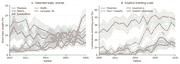
\includegraphics[width=\textwidth]{figures/06_key_trends.png}
\caption{Selected annual topics (A) and problem-framing cues (B). Topic shares describe mean NMF mixture weights; framing-cue rates describe overlapping textual matches. Bands are 95\% within-edition resampling intervals. They reflect composition sensitivity under fixed measures; they do not assess semantic validity.}
\label{fig:keytrends}
\end{figure*}

The language-modeling component reaches 20.5\% in 2026. Small early-period weights reflect shared language and text terms and are not evidence of early generative-AI research. A narrower lexical measure finds explicit LLM/generative-AI terms in 23/161 contributions in 2024 (14.3\%), 41/170 in 2025 (24.1\%), and 61/186 in 2026 (32.8\%). These counts measure visibility in the proceedings, not the prevalence of AI-generated content on social media.

\subsection{Different Problems within Community Research}
The community component's mean share changes little: 10.5\% [8.9, 12.2] in 2007--2011 and 10.0\% [8.8, 11.2] in 2022--2026, an endpoint difference of $-0.5$ percentage points [$-2.6$, 1.5]. Brackets throughout this section denote 95\% resampling intervals.

Governance cues within community-topic weight increase from 4.0\% [0.2, 8.8] to 34.3\% [27.0, 41.4], a difference of 30.3 points [21.8, 38.4]. Figure~\ref{fig:community} shows the annual series. It is uneven, but the endpoint contrast is large.

\begin{figure*}[t]
\centering
\includegraphics[width=\textwidth]{figures/07_community_governance.png}
\caption{Community research and governance framing. Panel A compares the community topic's share of all topic weight with the fraction of community-topic weight attached to papers containing governance cues; these series have different denominators. Panel B repeats the conditional rate after removing governance-matching features before projection onto the fixed topic basis. Bands describe composition sensitivity under the corresponding fixed representation.}
\label{fig:community}
\end{figure*}

Direct vocabulary overlap leaves the contrast largely intact. \emph{Moderation} is one of the community component's twenty leading terms and also matches the governance lexicon. Removing all seven governance-matching features changes the endpoint comparison to 3.6\% [0.1, 8.2] versus 32.5\% [25.3, 39.6], a difference of 28.9 points [20.6, 36.8]. Correlated vocabulary still links the two text-derived measures.

The same pattern survives stricter text checks. Restricting governance cues to the title and first 100 abstract words gives 2.5\% [0.0, 6.6] versus 25.8\% [18.7, 32.6], a difference of 23.2 points [15.1, 31.1]. Excluding papers whose only governance cues are \textit{moderate}, \textit{moderated}, \textit{moderates}, or \textit{moderating}, which often mark statistical or adjectival uses, gives 2.5\% [0.0, 6.6] versus 33.3\% [26.0, 40.4]. Refitting topics on titles and the first 100 abstract words leaves community share at 10.3\% and 9.7\% in the endpoint periods.

\subsection{Harm Framing and Measurement Sensitivity}
Across all contributions, harm/information-integrity cues increase from 6.2\% [3.9, 8.5] to 38.1\% [34.8, 41.2]. Governance cues increase from 1.3\% to 14.8\%, support/well-being cues from 1.3\% to 16.8\%, and prediction/classification cues from 36.3\% to 49.1\%. Table~\ref{tab:periods} uses the same four periods for all selected series.

\begin{table*}[t]
\small
\centering
\begin{tabular}{@{}lrrrr@{}}
\textbf{Measure} & \textbf{2007--2011} & \textbf{2012--2016} & \textbf{2017--2021} & \textbf{2022--2026} \\
\toprule
\rowcolmedium Contributions ($N$) & 386 & 503 & 488 & 762 \\
\hdashline
Networks / diffusion & 16.6 & 13.2 & 10.1 & 7.8 \\
Politics / polarization & 3.8 & 4.8 & 8.7 & 11.8 \\
Communities / participation & 10.5 & 9.2 & 10.0 & 10.0 \\
Health / social support & 2.8 & 4.4 & 6.2 & 6.3 \\
Prediction / classification cues & 36.3 & 42.9 & 47.7 & 49.1 \\
Measurement / validity cues & 8.5 & 15.1 & 15.0 & 18.1 \\
Explanation / intervention cues & 2.1 & 1.4 & 7.6 & 10.5 \\
Harm / integrity cues & 6.2 & 12.3 & 27.0 & 38.1 \\
Governance cues & 1.3 & 1.2 & 6.6 & 14.8 \\
Support / well-being cues & 1.3 & 5.8 & 9.8 & 16.8 \\
Governance within community-topic weight & 4.0 & 1.2 & 14.4 & 34.3 \\
\bottomrule
\end{tabular}
\caption{Selected measures across the same four five-edition periods. All values except $N$ are percentages. The first four rows of measures are mean topic weights; the next six are overlapping cue prevalences. The last row is conditional on community-topic weight. Headline resampling intervals are reported in the text.}
\label{tab:periods}
\end{table*}


\textbf{Abstract length.} Median abstract length increases from 113 words in 2007 to 190 in 2026. With titles plus the first 100 abstract words, harm-cue prevalence changes from 5.7\% [3.4, 8.0] to 31.9\% [28.7, 35.0]. With only the first 100 abstract words, it changes from 5.7\% [3.4, 8.0] to 31.0\% [27.8, 34.1]. The latter difference is 25.3 points [21.5, 29.2], smaller than the full-text difference. Mean harm-cue density also increases, from 0.10 to 0.78 matches per 100 title/abstract words.

\textbf{Historical vocabulary.} Adding trolling, flaming, and vandalism terms leaves the early-period harm estimate at 6.2\% and changes the last-period estimate to 38.3\%. Historical coverage remains uneven: 42.5\% of early contributions match none of the eight categories, compared with 14.0\% in the last period. Period-specific coding is needed to separate changing terminology from changes in framing. Appendix~\ref{app:sensitivity} reports the alternative measures for every period.

\subsection{Platform Context}
Figure~\ref{fig:platforms} addresses the platform dimension of RQ1. Blog mentions decrease from 35.2\% in 2007--2011 to 0.9\% in 2022--2026. Twitter-associated mentions reach a period peak of 45.7\% in 2012--2016 and decline to 24.8\% in 2022--2026. Reddit increases from 1.2\% in 2012--2016 to 15.4\% in 2022--2026. In 2026, Twitter/X and Reddit appear in 15.6\% and 16.1\% of contributions, respectively. These counts describe changing publication contexts; they do not measure platform replacement or equivalent data access.

\begin{figure*}[t]
\centering
\includegraphics[width=\textwidth]{figures/08_platform_shares.png}
\caption{Platform mentions in titles and abstracts for selected long-running contexts, with 95\% composition-resampling bands. Counts can overlap across platforms. The full dictionary contains twenty named families plus weblog terms (Appendix~\ref{app:platforms}).}
\label{fig:platforms}
\end{figure*}

Decentralized platforms have a small, uneven presence in this corpus. Mastodon is mentioned in 0, 3, 0, and 3 papers across 2023--2026; Bluesky in 0, 0, 2, and 3. Publication timing and title/abstract matching limit what these small counts can show.

Annual profiles do not support sharp phase boundaries: no boundary in the baseline five-segment model appears in more than 65\% of 200 resamples. We retain fixed comparison periods; Appendix~\ref{app:boundaries} reports the segmentation diagnostics.
 %2 page
% !TeX root = ../main.tex
\section{Methodological Developments and Recurring Questions}
\label{sec:methods_advances}
Selected studies show how methodological problems travel across platform generations. We organize them around sampling and representation, construct measurement, causal and experimental design, governance and disagreement, and research infrastructure. The examples illustrate design choices; they do not estimate conference-wide prevalence.

\subsection{Sampling and Representation}
Large datasets do not remove the need to specify whose behavior is observed. Early ICWSM work documented uneven Twitter demographics \citep{p14168}. Sampling later became an object of direct comparison: \citet{p14401} compared Twitter's sampled stream with Firehose data, and \citet{p7337} showed that fidelity depends on the scale and unit measured. Community selection raises a related problem. Demographic reweighting, for example, need not improve population prediction \citep{p19287}, while multilingual work broadens the contexts examined without automatically making them representative \citep{p19271}. Sampling should be assessed against a stated target population and question. AI assistance adds a prior question: whose behavior does the observed post reflect?

\subsection{Construct Measurement}
A trace can support more than one interpretation. In 2007, \citet{icwsm2007_paper19} combined network analysis with a survey of blogging relationships, using evidence beyond the trace to assess what links and comments represented. Later work distinguished follower counts from retweet- and mention-based influence \citep{p14033}.

Text measures make the same problem visible at scale. Dictionary estimates of regional well-being can diverge sharply from survey measures across populations \citep{jaidka2020estimating}. Recent ICWSM work finds similar limits when measuring moral foundations in Chinese: local lexicons lose cultural information, while multilingual and large language models still require human validation \citep{p42650}. LLM-simulated respondents can also distort relationships found in human survey data \citep{p42652}. Assisted writing adds another layer because it can change observed language without the same change in the person \citep{hohenstein2023}.

\subsection{Causal and Experimental Design}
\label{sec:causal}
Social media histories provide pretreatment language and behavior, but causal claims require a defensible comparison. Table~\ref{tab:designs} contrasts randomized interventions, quasi-random assignment, difference-in-differences, estimator evaluation, and matching-based designs represented in ICWSM.

\begin{table*}[t]
\centering
\small
\begin{tabular}{@{}p{.16\textwidth}p{.20\textwidth}p{.28\textwidth}p{.28\textwidth}@{}}
\textbf{Design} & \textbf{ICWSM Example} & \textbf{Requires} & \textbf{Leaves open} \\
\toprule
Randomized intervention & Reconsideration prompts on Twitter \citep{p19308} & Random assignment supports a comparison of eligible users assigned to receive the prompt. & Classifier-defined eligibility and outcomes; transfer beyond English replies and the study setting. \\
\hdashline
Quasi-random assignment & Civil communication on Roblox \citep{p31365} & Residual stochasticity in matchmaking assignment acts as a quasi-randomization mechanism for the analyzed server comparisons. & Other server properties may co-vary with civility; validity and transfer of the local comparison. \\
\hdashline
Matching and difference-in-differences & Fringe-platform participation \citep{p22184} & Comparable untreated trends after matching; no differential concurrent changes explaining the contrast. & Selective migration, cross-platform linkage, and changing composition or exposure. \\
\hdashline
Text-adjustment evaluation & Known-effect benchmark tasks \citep{p19362} & Effects are known under the benchmark's construction, enabling comparisons of estimators. & Performance under the benchmark need not transfer to an unknown real-world assignment process. \\
\hdashline
Propensity-score stratification & Support language and college alcohol mentions \citep{p14891,p15012} & Conditional exchangeability, overlap, consistent exposure definitions, and appropriate timing. & Unmeasured circumstances and linguistic proxies; balance alone cannot establish exchangeability. \\
\hdashline
Two-tier matching & Counseling recommendations \citep{p15016} & Observed behavioral and linguistic covariates suffice to adjust confounding for the defined exposure. & Commenting differs from reading a post or receiving counseling; uptake remains unobserved. \\
\hdashline
Outcome-oriented case--control comparison & Psychosocial outcomes on TalkLife \citep{p7326} & Comparisons are conditional on subsequent outcomes and observed baseline groups. & Outcome selection and residual confounding; does not itself identify an assigned intervention's effect. \\
\hdashline
Randomization under interference & Cascade-based design \citep{p31322} & The network and diffusion model adequately describe relevant interference in the evaluated setting. & Misspecified or changing networks; simulation performance does not establish a field effect. \\
\bottomrule
\end{tabular}
\caption{Causal-inference designs in ICWSM research, with the conditions each design requires and the questions it leaves open. Examples illustrate each design's use.}
\label{tab:designs}
\end{table*}


The examples make exposure definitions and comparison groups explicit. Engagement with a counseling post, for example, differs from reading it or receiving counseling. Matching addresses measured differences, while unmeasured confounding can remain. Temporal comparisons require an appropriate counterfactual trajectory, and network settings raise interference questions. \citet{p19362} also show why text-adjustment estimators need evaluation against known-effect tasks. Suggested replies and automated moderation create the same design problem: studies need explicit exposures and credible comparisons, with spillovers addressed when interactions cross users.

\subsection{Governance and Disagreement}
Questions about judgment and authority appear throughout ICWSM's history. Automatic comment moderation appeared in the inaugural proceedings \citep{icwsm2007_paper59}, and Wikipedia work examined governance through promotion processes \citep{p14013}. Later research connected community rules to perceived governance \citep{p15033}. These examples place classification decisions inside the institutions and norms that give them meaning.

LLM-based annotation and moderation extend those questions to model-generated judgments. Studies document LLM annotation bias \citep{p35879}, moderator disagreement \citep{p42625}, and how LLMs apply Wikipedia neutrality norms \citep{p42630}. A model's agreement with a reference label depends on whose judgment the label represents. Evaluations should document whose labels define the reference and where those decisions are used.

\subsection{Research Infrastructure}
Tools and datasets shape which studies can be conducted and repeated. CrisisLex supported research on crisis communication \citep{p14538}; the Pushshift Reddit dataset expanded access to community activity \citep{p7347}; Media Cloud and the Methods Hub support news archives and executable methods \citep{p18127,p42804}. Infrastructure also sets conditions on use. Researcher access under the Digital Services Act makes those constraints part of the research question \citep{p42671}, while work on generative AI in crowdwork raises provenance concerns for apparently human-produced inputs \citep{p31452}. In AI-mediated settings, provenance includes model versions and whether content was composed, edited, selected, or generated.
 %3 page
% !TeX root = ../main.tex
\section{Discussion}
Two decades of ICWSM show substantial platform turnover without erasing familiar research problems. Community research makes this visible: its topic share changes little across the endpoint periods, while governance cues become much more common. The literature shows why that distinction matters. Sampling still determines whose behavior enters a study; traces still need construct validation; causal claims still depend on comparison design; moderation still embeds judgment; and data access still constrains what researchers can observe. AI changes each of these conditions, especially the provenance of language and exposure.

\paragraph{Following questions within topics.}
Topical continuity can conceal changes in what researchers seek to explain or improve. Retrospectives can connect subjects with research questions, designs, and intended beneficiaries. The weak stability of our phase boundaries favors overlapping interests over sharply separated eras. Historical interviews and archival work could explain changes that publication profiles cannot.

\paragraph{Making methodological comparisons reusable.}
Table~\ref{tab:checklist} turns recurring design questions into reporting items. A later reader should be able to judge whether a finding still applies after a platform, access regime, or content-production process changes. The checklist is a reporting aid; it does not certify that an assumption holds.

\begin{table*}[t]
\small
\centering
\begin{tabular}{@{}p{.20\textwidth}p{.73\textwidth}@{}}
\textbf{Reporting item} & \textbf{Information to provide} \\
\toprule
Target population & Who or what is the study about? Describe observed users, communities, languages, dates, and exclusions; distinguish the sample from the target population. \\
\rowcollight Question and estimand & State the descriptive quantity or causal contrast, unit of analysis, exposure, outcome, and time horizon. Specify whose effect is estimated. \\
Constructs and measures & Explain why each trace or label measures the intended construct. Report validation, disagreements, missingness, and relevant subgroup or period differences. \\
\rowcollight Collection and provenance & Record interfaces, sampling rules, access restrictions, deletion or attrition, and data and model versions. Document content-production processes where known. \\
Assignment and timing & Describe how exposure arises, the comparison group, and the ordering of covariates, treatment, and outcomes. Identify concurrent events and possible spillovers. \\
\rowcollight Adjustment and overlap & Justify pretreatment covariates, including text features. Report balance, overlap, exclusions, and any change in the target population after adjustment. \\
Sensitivity and uncertainty & State assumptions and plausible failures. Use appropriate sensitivity analyses, alternative measures, placebo or negative-control comparisons, and uncertainty estimates. \\
\rowcollight Interpretation and reuse & Separate prediction, association, and causal interpretation. State limits of transfer and provide reusable code, definitions, and access information when possible. \\
\bottomrule
\end{tabular}
\caption{A reporting checklist for studies using social media observations. Items should be applied to the study's question and design, with non-applicable items explained. The checklist is a reporting aid, not a quality score or a substitute for validation.}
\label{tab:checklist}
\end{table*}


\paragraph{Interpreting AI-mediated interaction.}
AI-mediated communication includes systems that modify, augment, or generate messages on a person's behalf \citep{hancock2020}. A post can now reflect a person's intentions, model suggestions, interface defaults, and platform rules. Final text alone may no longer reveal who composed a message or whose attention it represents.

This matters for measures that infer attitudes, distress, or social support from text. Experiments with suggested replies show that assistance can change language and interpersonal evaluations, while suspected assistance can lower how a partner is perceived \citep{hohenstein2023}. Language quality, perceived care, and interaction benefit should be measured separately. Our LLM-related publication counts motivate these questions; they do not measure how much social media communication is AI-mediated.

AI mediation also changes exposure. A person may encounter generated replies, ranking decisions, and moderation actions that change over time. Studies can record whether people composed, edited, selected, or only received generated content, together with system versions and interaction context. Consented process records, participant accounts, and interface experiments can provide evidence that final text cannot recover. These records support questions about delegation, trust, social obligation, and community norms even when human and machine contributions cannot be cleanly separated.

\paragraph{Preserving comparisons across changing systems.}
Platform access, model versions, and content-production processes can change both behavior and observation. Recording validation evidence, disagreement, collection conditions, and system versions lets later researchers assess whether an earlier finding transfers. Cumulative comparisons depend on preserving the conditions under which a claim was supported.
 %2 page
% !TeX root = ../main.tex
\section{Limitations and Future Directions}
Our topic labels and framing cues approximate the constructs of interest. Components can combine domains, tasks, and writing styles; a cue can describe background. Length, vocabulary, and strict-cue checks address specific artifacts but cannot establish precision or recall. Independent judgments are needed for positive and negative cases. Appendix~\ref{app:validation} specifies a stratified coding and intrusion-test protocol; those results are not incorporated in the present estimates.

The corpus combines publication formats whose representation may change over time. Including datasets and demonstrations captures research infrastructure, but their abstracts may emphasize different problems from full papers. A full-paper-only analysis should use verified proceedings section labels and compare like formats within the same editions. Reconciliation of every issue and track would also strengthen the coverage audit.

The methodological examples come from an exploratory bibliography and cannot estimate the prevalence or influence of a design. A structured full-text review that samples beyond cue-positive abstracts and documents disconfirming cases would strengthen the synthesis.

Publication year is an imperfect proxy for when a study was conceived or its data were collected. Topic changes and segmentation boundaries do not identify why research interests changed. Platform contexts also changed over this period, so part of the community-governance contrast may reflect which platforms the conference studied. Separating platform composition from changing problem framing requires platform-stratified analysis. Our resampling intervals hold measurements fixed and therefore exclude model and interpretation uncertainty. Future work could combine validated coding, alternative representations, citation analysis, and accounts from researchers. For AI-mediated interaction, publication trends also need direct evidence about how people and communities use the systems being studied.
 %2 page
% !TeX root = ../main.tex
\section{Conclusion}
Across 2,139 contributions and twenty ICWSM editions, we find platform turnover alongside recurring research questions. Community research stays near one tenth of topic weight, while governance cues within it rise from 4.0\% to 34.3\%. The contrast remains after removing shared governance vocabulary, shortening abstracts, and tightening the governance cue. Selected studies across the conference repeatedly confront problems of representation, measurement, causal comparison, governance, and data access. Platforms change; the questions recur. AI systems now participate in producing, ranking, and moderating online interaction, making the provenance of both content and exposure part of the evidence. We will release the corpus and analysis materials upon publication; the reporting checklist provides a common record for future comparisons.
 %2 page
% !TeX root = ../main.tex
\section*{Ethical Considerations}
Our study uses public scholarly publications and Crossref metadata. It involves no new recruitment or analysis of individuals' social media posts. We retain author names for bibliographic attribution and do not infer sensitive attributes or rank researchers. Publication counts and framing cues could be misused as indicators of research quality or community concern. We reduce this risk through explicit measurement definitions, counterexamples, and sensitivity analyses. Upon publication, we will release bibliographic metadata, machine-readable derived measurements, analysis code, dictionaries, and documentation with persistent identifiers, source links, and a data card describing provenance and reuse constraints. Crossref bibliographic metadata is reusable without restriction, while abstracts remain subject to publisher or author copyright.\footnote{\url{https://www.crossref.org/documentation/retrieve-metadata/}} We will not redistribute source papers or bulk abstracts.
 %2 page
% !TeX root = ../main.tex
\section*{Acknowledgements}
OpenAI's ChatGPT and Codex, and Anthropic's Claude, were used to assist with literature retrieval and synthesis, corpus assembly, analysis code, figures and tables, references, AI-assisted inspection of topic labels and lexical cues, source checking, and manuscript drafting and revision. Quantitative results were computed with the Python analysis scripts. The authors directed the research design, reviewed the generated material, and take responsibility for the final content.

% \input{sections/9.0conclusions.tex} %2 page

% Use \bibliography{yourbibfile} instead or the References section will not appear in your paper
\bibliography{references}

\section*{Ethics Checklist}

\begin{enumerate}

\item For most authors...
\begin{enumerate}
    \item Would answering this research question advance science without violating social contracts, such as violating privacy norms, perpetuating unfair profiling, exacerbating the socio-economic divide, or implying disrespect to societies or cultures?
    \answerYes{Yes. The study analyzes public scholarly publications and metadata. It involves no new participants and no analysis of individuals' social media posts (see Ethical Considerations).}
  \item Do your main claims in the abstract and introduction accurately reflect the paper's contributions and scope?
    \answerYes{Yes. The abstract and introduction describe topics and problem-framing cues at the scope supported by the analysis, and Section~3 states that the methodological examples are illustrative.}
   \item Do you clarify how the proposed methodological approach is appropriate for the claims made?
    \answerYes{Yes. Section~3 explains what topic mixtures and framing cues measure, their limitations, the sensitivity analyses, and how the literature examples were selected. Appendices~B and C provide the topic terms and framing codebook.}
   \item Do you clarify what are possible artifacts in the data used, given population-specific distributions?
    \answerYes{Yes. We examine abstract length, historical vocabulary, shared vocabulary between topics and framing cues, paper composition across editions, and corpus coverage (Sections~3, 4, and 7; Appendix~D).}
  \item Did you describe the limitations of your work?
    \answerYes{Yes. See Section~7.}
  \item Did you discuss any potential negative societal impacts of your work?
    \answerYes{Yes. Publication counts and textual cues could be misread as indicators of research quality or community concern (see Ethical Considerations).}
  \item Did you discuss any potential misuse of your work?
    \answerYes{Yes. We caution against using the measures to rank researchers or judge research quality (see Ethical Considerations).}
  \item Did you describe steps taken to prevent or mitigate potential negative outcomes of the research, such as data and model documentation, data anonymization, responsible release, access control, and the reproducibility of findings?
    \answerYes{Yes. We provide explicit measurement definitions, sensitivity analyses, a codebook, and an independent validation protocol, and we document provenance and reuse constraints for the planned release (Section~3; Appendices~C, D, and F; Ethical Considerations). We do not infer sensitive attributes of authors.}
  \item Have you read the ethics review guidelines and ensured that your paper conforms to them?
    \answerYes{Yes.}
\end{enumerate}

\item Additionally, if your study involves hypotheses testing...
\begin{enumerate}
  \item Did you clearly state the assumptions underlying all theoretical results?
    \answerNA{NA. The study is descriptive and does not test hypotheses or develop theoretical results.}
  \item Have you provided justifications for all theoretical results?
    \answerNA{NA.}
  \item Did you discuss competing hypotheses or theories that might challenge or complement your theoretical results?
    \answerNA{NA.}
  \item Have you considered alternative mechanisms or explanations that might account for the same outcomes observed in your study?
    \answerNA{NA. We nevertheless examine measurement-based alternative explanations for the observed patterns, including abstract length and shared vocabulary (Section~3; Appendix~D).}
  \item Did you address potential biases or limitations in your theoretical framework?
    \answerNA{NA.}
  \item Have you related your theoretical results to the existing literature in social science?
    \answerNA{NA.}
  \item Did you discuss the implications of your theoretical results for policy, practice, or further research in the social science domain?
    \answerNA{NA.}
\end{enumerate}

\item Additionally, if you are including theoretical proofs...
\begin{enumerate}
  \item Did you state the full set of assumptions of all theoretical results?
    \answerNA{NA.}
  \item Did you include complete proofs of all theoretical results?
    \answerNA{NA.}
\end{enumerate}

\item Additionally, if you ran machine learning experiments...
\begin{enumerate}
  \item Did you include the code, data, and instructions needed to reproduce the main experimental results (either in the supplemental material or as a URL)?
    \answerNo{No. The corpus, derived measurements, analysis code, and documentation will be released upon publication; no anonymous release is included with this review submission.}
  \item Did you specify all the training details (e.g., data splits, hyperparameters, how they were chosen)?
    \answerYes{Yes. Section~3 reports the TF--IDF representation, vocabulary threshold, number of components, initialization, random seed, iteration limit, and alternative specifications. The unsupervised analysis uses no data splits.}
  \item Did you report error bars (e.g., with respect to the random seed after running experiments multiple times)?
    \answerYes{Yes. We report 95\% within-edition resampling intervals from 2,000 resamples (Sections~3 and 4; Figures~1--3) and compare alternative component counts and random initializations.}
  \item Did you include the total amount of compute and the type of resources used (e.g., type of GPUs, internal cluster, or cloud provider)?
    \answerNo{No. Hardware-specific resources and total compute were not recorded.}
  \item Do you justify how the proposed evaluation is sufficient and appropriate to the claims made?
    \answerYes{Yes. Sections~3 and 7 state which claims the current evidence supports and which require independent validation. Appendix~F specifies that validation protocol.}
  \item Do you discuss what is ``the cost`` of misclassification and fault (in)tolerance?
    \answerYes{Yes. We discuss how incidental cue matches and missed concerns affect interpretation of prevalence estimates (Sections~3, 4, and 7; Appendix~C) and how the measures could be misread as quality indicators (Ethical Considerations).}
\end{enumerate}

\item Additionally, if you are using existing assets (e.g., code, data, models) or curating/releasing new assets...
\begin{enumerate}
  \item If your work uses existing assets, did you cite the creators?
    \answerYes{Yes. We cite Crossref, the AAAI proceedings archive, the official ICWSM 2007 program, and the publications discussed in the paper.}
  \item Did you mention the license of the assets?
    \answerYes{Yes. Crossref bibliographic metadata is reusable without restriction, while abstracts remain subject to publisher or author copyright. We therefore do not plan to redistribute source papers or bulk abstracts (see Ethical Considerations).}
  \item Did you include any new assets in the supplemental material or as a URL?
    \answerNo{No. The corpus, derived measurements, analysis code, and documentation will be released upon publication.}
  \item Did you discuss whether and how consent was obtained from people whose data you're using/curating?
    \answerYes{Yes. The study uses published scholarly metadata and involves no human participants. No additional consent was obtained, and author names are retained only for bibliographic attribution (see Ethical Considerations).}
  \item Did you discuss whether the data you are using/curating contains personally identifiable information or offensive content?
    \answerYes{Yes. The only personal information is author names in bibliographic records. We do not infer sensitive attributes or rank researchers (see Ethical Considerations).}
  \item If you are curating or releasing new datasets, did you discuss how you intend to make your datasets FAIR (see \citet{fair})?
    \answerYes{Yes. The planned release will use persistent identifiers, source links, machine-readable derived measurements, documented inclusion decisions, and provenance and reuse documentation (see Ethical Considerations).}
  \item If you are curating or releasing new datasets, did you create a Datasheet for the Dataset (see \citet{gebru2021datasheets})?
    \answerNo{No. A data card will accompany the release upon publication.}
\end{enumerate}

\item Additionally, if you used crowdsourcing or conducted research with human subjects...
\begin{enumerate}
  \item Did you include the full text of instructions given to participants and screenshots?
    \answerNA{NA. The reported analyses involve no participants. Appendix~F specifies a future independent coding protocol; its results are not reported in this paper.}
  \item Did you describe any potential participant risks, with mentions of Institutional Review Board (IRB) approvals?
    \answerNA{NA.}
  \item Did you include the estimated hourly wage paid to participants and the total amount spent on participant compensation?
    \answerNA{NA.}
  \item Did you discuss how data is stored, shared, and deidentified?
    \answerNA{NA.}
\end{enumerate}

\end{enumerate}


% \cleardoublepage\makeatletter\@openrightfalse\makeatother
% \cleardoublepage\makeatletter\makeatother
% \let\clearpage\relax
% \openright
\appendix
% !TeX root = ../main.tex
\onecolumn
\setcounter{figure}{0}
\setcounter{table}{0}
\renewcommand{\thefigure}{A\arabic{figure}}
\renewcommand{\thetable}{A\arabic{table}}
\section{Corpus and Platform Dictionaries}
\label{app:corpus}
Figure~\ref{fig:corpus} reports indexed contributions by edition. These are publication counts, not submission or acceptance counts. The main analysis includes all retained main-conference formats.
\begin{figure}[ht]
\centering
\includegraphics[width=.75\textwidth]{figures/01_corpus.png}
\caption{Annual contributions in the retrieved corpus.}
\label{fig:corpus}
\end{figure}
\subsection{Platform families}
\label{app:platforms}
The twenty named platform families are Twitter/X, Reddit, Facebook, Wikipedia, YouTube, Instagram, TikTok/Douyin, Weibo, WeChat, WhatsApp, Telegram, Gab, 4chan, Parler, Mastodon, Bluesky, Flickr, Digg, MySpace, and StackOverflow. A separate weblog indicator matches blogs, weblogs, blogging, bloggers, and blogosphere. Twitter includes tweets and retweets; Reddit includes subreddit and redditor variants; Wikipedia includes Wikipedian variants. StackOverflow allows a space between the two words. Seven X-only cases, identified through AI-assisted inspection, supplement the Twitter vocabulary. All other named families use the explicit name, with case-insensitive word boundaries. The regular expressions used in the analysis will be released upon publication and provide the exact specification. Rates count mentions, can overlap, and do not establish data use.

\section{Topic Components and Complete Distributions}
\label{app:topics}
Topic labels describe one exploratory 15-component NMF representation. Table~\ref{tab:topicterms} lists each component's twenty highest-weight terms in order. Figure~\ref{fig:topicsproblems} orders rows by the difference between the last and first fixed periods, from the largest increase to the largest decrease, separately for topics and framings. Component weights and cue prevalences have different denominators.
\begingroup
\small
\begin{longtable}{@{}p{.05\textwidth}p{.22\textwidth}p{.65\textwidth}@{}}
\caption{NMF components and top terms, ordered by component identifier.}\label{tab:topicterms}\\
\toprule
ID & Interpretive label & Twenty highest-weight terms \\
\midrule
\endfirsthead
\toprule
ID & Interpretive label & Twenty highest-weight terms \\
\midrule
\endhead
\bottomrule
\endfoot
T00 & Networks, diffusion, recommendation & diffusion, influence, link, graph, structure, recommendation, nodes, problem, prediction, links, cascades, node, systems, graphs, real, items, spread, popularity, link prediction, algorithms \\ \addlinespace
T01 & Conventional classification & learning, classification, features, detection, machine, machine learning, performance, task, accuracy, supervised, art, state art, training, state, framework, labeled, reviews, f1, problem, existing \\ \addlinespace
T02 & News and journalism & news, articles, news articles, article, outlets, sources, news outlets, fake, news sources, coverage, fake news, stories, news article, comments, misinformation, bias, source, readers, sharing, local news \\ \addlinespace
T03 & Language modeling and generative AI & llms, language, llm, ai, human, language llms, generated, gpt, tasks, fine, performance, text, reasoning, english, languages, framework, bias, biases, natural language, detection \\ \addlinespace
T04 & Pandemics and vaccination & covid, covid 19, 19, pandemic, 19 pandemic, vaccine, anti, misinformation, vaccination, vaccines, related, impact, health, stance, concerns, narratives, public, understand, population, conspiracy \\ \addlinespace
T05 & Politics and polarization & political, election, accounts, elections, polarization, discourse, party, politicians, partisan, campaigns, presidential, public, parties, leaning, engagement, right, political discourse, campaign, topics, candidates \\ \addlinespace
T06 & Sentiment and opinion mining & sentiment, topic, topics, text, sentiments, opinion, positive, negative, opinions, corpus, words, polarity, word, set, mood, semantic, emotions, related, mining, terms \\ \addlinespace
T07 & Communities and participation & communities, community, members, group, groups, participation, activity, subreddits, behavior, moderation, work, engagement, discussion, interactions, active, patterns, success, subreddit, dynamics, effect \\ \addlinespace
T08 & Events and collective attention & events, event, real, world, real world, time, real time, world events, messages, stream, response, summarization, event detection, crisis, temporal, streams, disaster, detection, short, relevant \\ \addlinespace
T09 & Identity and self-presentation & gender, profiles, people, profile, personality, self, age, friends, differences, personal, female, women, attributes, men, traits, male, likely, demographic, interactions, groups \\ \addlinespace
T10 & Search, Q\&A, and tagging & question, search, questions, answering, answer, answers, quality, question answering, tagging, tags, systems, queries, engine, search engine, community question, engines, search engines, knowledge, expertise, tag \\ \addlinespace
T11 & Health and social support & health, mental, mental health, support, posts, self, individuals, depression, emotional, public, post, risk, effects, findings, stress, public health, related, treatment, examine, discuss \\ \addlinespace
T12 & Hateful and abusive speech & hate, speech, hate speech, speech detection, detection, hateful, moderation, targets, target, attacks, comments, replies, toxic, offensive, understanding, harassment, automatic, language, conversations, toxicity \\ \addlinespace
T13 & Visual and multimodal media & videos, video, images, memes, visual, meme, image, multimodal, popularity, misinformation, channels, sharing, creators, popular, whatsapp, shared, channel, metadata, short, audio \\ \addlinespace
T14 & Location and mobility & location, mobility, urban, check, patterns, foursquare, city, locations, temporal, services, cities, spatial, places, geographic, human mobility, ins, check ins, behavior, time, mobile \\ \addlinespace
\end{longtable}
\endgroup

\begin{figure}[p]
\centering
\includegraphics[width=\textwidth]{figures/04_topics_problems.png}
\caption{Complete annual topic shares and framing-cue prevalences, ordered by endpoint-period change. Topic shares sum to 100\%; framing categories overlap. No historical phase boundaries are imposed.}
\label{fig:topicsproblems}
\end{figure}
\section{Framing Codebook}
\label{app:codebook}
The definitions distinguish an intended research problem from the lexical rule used to approximate it. Example cues are illustrative; the regular expressions used in the analysis specify matching exactly. A cue can be incidental, and an absent cue does not establish an absent concern. Categories are not mutually exclusive.
\begingroup
\small
\begin{longtable}{@{}p{.20\textwidth}p{.46\textwidth}p{.26\textwidth}@{}}
\caption{Definitions and example lexical cues for the eight overlapping framing cues.}\label{tab:codebook}\\
\toprule
Category & Definition and scope limitation & Example cues \\
\midrule
\endfirsthead
\toprule
Category & Definition and scope limitation & Example cues \\
\midrule
\endhead
\bottomrule
\endfoot
P1 Structure and diffusion & Explicit framing of relational structure, diffusion, contagion, social influence, collective dynamics, or community formation. Does not identify every explanatory study of collective behavior. & diffusion; cascades; social ties; homophily \\ \addlinespace
P2 Prediction and classification & Explicit prediction, forecasting, classification, detection, or recommendation terminology. May match a prediction or detection task that a paper critiques rather than performs. & prediction; forecasting; classification; detection \\ \addlinespace
P3 Measurement and validity & Explicit validation, sampling, representation, reliability, ground truth, reproducibility, or measurement-error terminology. Routine uses of the verb measure alone do not qualify. Validation and reliability can refer to routine evaluation or background discussion, not a central measurement contribution. & validity; sampling; ground truth; reliability \\ \addlinespace
P4 Explanation and intervention & Explicit causation, intervention, recognizable experimental-design terminology, causal/social mechanisms, or theory testing. Generic mechanism and theoretical implication mentions are excluded. Theory, mechanism, or causal language does not establish a valid causal design. & causal; intervention; randomized; propensity score \\ \addlinespace
P5 Harm and information integrity & Explicit information-integrity, abuse, discrimination, privacy-risk, spam, or other harm framing. Includes descriptive and technical work about harm, without inferring the authors' normative commitments. & misinformation; spam; harassment; privacy; harm \\ \addlinespace
P6 Governance and participation & Explicit moderation, governance, censorship, enforcement, platform rules, or community norms. Does not capture every study of participation; moderation can also be mentioned as background. & moderation; governance; censorship; community rules \\ \addlinespace
P7 Support and well-being & Explicit human-health, care, distress, social-support, or well-being framing. The bare word health is excluded to reduce organizational-health metaphors. A health mention does not establish a clinical outcome or a supportive intervention. & mental health; caregiving; depression; social support \\ \addlinespace
P8 Resources and research access & Explicit nearby provision of data/tools or data-access and research-infrastructure terminology. Generic API and publicly available mentions alone do not qualify. A paper can provide a tool without belonging to a dataset or demonstration track. & researcher access; open-source; releases a dataset \\ \addlinespace
\end{longtable}
\endgroup

\section{Sensitivity Results}
\label{app:sensitivity}
Table~\ref{tab:sensitivity} reports the harm and community-governance checks using the four main comparison periods. Density is the mean of paper-level cue matches divided by title/abstract word count and multiplied by 100; it is not a paper prevalence. The historical union adds trolling, flaming, and vandalism terms to all editions. Spam is already in the baseline harm lexicon. The strict governance cue excludes papers whose only matches are \emph{moderate}, \emph{moderated}, \emph{moderates}, or \emph{moderating}.
\begingroup
\small
\begin{longtable}{@{}p{.36\textwidth}rrrr@{}}
\caption{Sensitivity estimates. All rows except cue density are percentages.}\label{tab:sensitivity}\\
\toprule
Measure & 2007--11 & 2012--16 & 2017--21 & 2022--26 \\
\midrule
\endfirsthead
\toprule
Measure & 2007--11 & 2012--16 & 2017--21 & 2022--26 \\
\midrule
\endhead
\bottomrule
\endfoot
Harm: full title/abstract & 6.2 & 12.3 & 27.0 & 38.1 \\ \addlinespace
Harm: title + first 100 abstract words & 5.7 & 9.5 & 22.7 & 31.9 \\ \addlinespace
Harm: first 100 abstract words only & 5.7 & 8.7 & 21.9 & 31.0 \\ \addlinespace
Harm: historical union & 6.2 & 12.3 & 27.9 & 38.3 \\ \addlinespace
Harm: mean matches / 100 words & 0.10 & 0.23 & 0.54 & 0.78 \\ \addlinespace
Governance within community topic & 4.0 & 1.2 & 14.4 & 34.3 \\ \addlinespace
Governance after feature masking & 3.6 & 1.1 & 13.4 & 32.5 \\ \addlinespace
Governance within community: title + first 100 words & 2.5 & 0.8 & 8.8 & 25.8 \\ \addlinespace
Governance within community: first 100 abstract words & 2.5 & 0.8 & 7.4 & 25.6 \\ \addlinespace
Governance within community: strict cue & 2.5 & 0.5 & 12.5 & 33.3 \\ \addlinespace
Governance cues overall: strict cue & 0.8 & 0.6 & 5.5 & 13.1 \\ \addlinespace
\end{longtable}
\endgroup

\subsection{Direct term overlap}
Table~\ref{tab:overlap} gives the number of each topic's top twenty terms matched by each framing expression. For the community component, only \emph{moderation} matches the governance expression. The vocabulary-removal analysis masks every governance-matching unigram or bigram in the fitted vocabulary, not just the top twenty terms. The complete term-level overlap record will be released with the analysis materials upon publication.
\begingroup
\small
\begin{longtable}{@{}lrrrrrrrr@{}}
\caption{Counts of top-twenty topic terms matched by each framing lexicon. These are literal term matches, not measures of semantic independence.}\label{tab:overlap}\\
\toprule
Topic & P1 & P2 & P3 & P4 & P5 & P6 & P7 & P8 \\
\midrule
\endfirsthead
\toprule
Topic & P1 & P2 & P3 & P4 & P5 & P6 & P7 & P8 \\
\midrule
\endhead
\bottomrule
\endfoot
T00 & 2 & 3 & 0 & 0 & 0 & 0 & 0 & 0 \\ \addlinespace
T01 & 0 & 2 & 0 & 0 & 0 & 0 & 0 & 0 \\ \addlinespace
T02 & 0 & 0 & 0 & 0 & 2 & 0 & 0 & 0 \\ \addlinespace
T03 & 0 & 1 & 0 & 0 & 0 & 0 & 0 & 0 \\ \addlinespace
T04 & 0 & 0 & 0 & 0 & 2 & 0 & 7 & 0 \\ \addlinespace
T05 & 0 & 0 & 0 & 0 & 0 & 0 & 0 & 0 \\ \addlinespace
T06 & 0 & 0 & 0 & 0 & 0 & 0 & 0 & 0 \\ \addlinespace
T07 & 0 & 0 & 0 & 0 & 0 & 1 & 0 & 0 \\ \addlinespace
T08 & 0 & 2 & 0 & 0 & 0 & 0 & 0 & 0 \\ \addlinespace
T09 & 0 & 0 & 0 & 0 & 0 & 0 & 0 & 0 \\ \addlinespace
T10 & 0 & 0 & 0 & 0 & 0 & 0 & 0 & 0 \\ \addlinespace
T11 & 0 & 0 & 0 & 0 & 0 & 0 & 3 & 0 \\ \addlinespace
T12 & 0 & 2 & 0 & 0 & 5 & 1 & 0 & 0 \\ \addlinespace
T13 & 0 & 0 & 0 & 0 & 1 & 0 & 0 & 0 \\ \addlinespace
T14 & 0 & 0 & 0 & 0 & 0 & 0 & 0 & 0 \\ \addlinespace
\end{longtable}
\endgroup

\section{Exploratory Temporal Segmentation}
\label{app:boundaries}
For segmentation only, we normalize annual overlapping framing-cue rates together with an unmatched category. We concatenate square-root topic and framing shares, weighting the axes equally, and minimize within-segment squared deviation. Each edition has equal weight in this diagnostic. This differs from pooling papers within the fixed periods used in the main analysis.

The baseline five-segment solution with a three-edition minimum has starts in 2007, 2011, 2017, 2021, and 2024. Its full partition recurs in 29/200 resamples (14.5\%). Exact boundary frequencies are given below. The baseline minimum makes 2024 the latest possible final start, so its apparent recurrence cannot establish a recent historical break. A second analysis uses the same 200 newly sampled paper compositions to compare two- and three-edition minima. It admits a 2025 start, which appears in 47/200 resamples (23.5\%). These are conditional exact-year frequencies, not confidence levels for historical events.
\begingroup
\small
\begin{longtable}{@{}lrrr@{}}
\caption{Exact-year boundary recurrence (percent) under five-segment joint profiles. A dash marks a boundary disallowed by the minimum-length rule. The two new columns use identical resampled paper compositions.}\label{tab:boundaries}\\
\toprule
Boundary start & Baseline 200; min. 3 & New 200; min. 3 & Same new 200; min. 2 \\
\midrule
\endfirsthead
\toprule
Boundary start & Baseline 200; min. 3 & New 200; min. 3 & Same new 200; min. 2 \\
\midrule
\endhead
\bottomrule
\endfoot
2009 & -- & -- & 21.5 \\ \addlinespace
2010 & 39.5 & 39.0 & 33.0 \\ \addlinespace
2011 & 56.5 & 59.0 & 54.5 \\ \addlinespace
2012 & 3.5 & 1.5 & 28.0 \\ \addlinespace
2013 & 19.5 & 20.5 & 5.0 \\ \addlinespace
2014 & 16.5 & 13.0 & 8.0 \\ \addlinespace
2015 & 6.5 & 9.0 & 5.5 \\ \addlinespace
2016 & 1.0 & 2.5 & 0.5 \\ \addlinespace
2017 & 54.0 & 53.0 & 55.5 \\ \addlinespace
2018 & 34.0 & 34.0 & 31.5 \\ \addlinespace
2019 & 11.5 & 12.5 & 23.0 \\ \addlinespace
2020 & 21.5 & 19.5 & 14.5 \\ \addlinespace
2021 & 65.0 & 65.5 & 70.5 \\ \addlinespace
2022 & 7.0 & 5.5 & 4.0 \\ \addlinespace
2023 & 0.0 & 0.0 & 0.0 \\ \addlinespace
2024 & 64.0 & 65.5 & 21.5 \\ \addlinespace
2025 & -- & -- & 23.5 \\ \addlinespace
\end{longtable}
\endgroup

We also retain results for three, four, and five segments and topic-only, framing-only, and joint representations. The segment count is not selected by an external validation criterion. Changes in component count and initialization can move boundaries. We therefore do not name a definitive sequence of five phases or use it to calculate the headline period comparisons. Broad emphases can overlap even when a segmentation algorithm must assign each year to one interval.

\section{Independent Validation Protocol}
\label{app:validation}
The framing-validation protocol samples 20 papers per edition (400 total), without restricting to cue-positive cases. Two coders independently judge whether each abstract expresses a substantive objective matching each category, distinguishing central or evaluated concerns from incidental background. Multiple categories are allowed; uncertain cases receive a separate flag. The protocol materials withhold automatic predictions. Source links can reveal bibliographic identity; an optional local reader also withholds author and edition information.

Report per-category Cohen's $\kappa$, raw agreement, and positive-label counts overall and by fixed period. After preserving the independent ratings, adjudicate disagreements and uncertainty. Compare the frozen cues with those adjudicated judgments, reporting precision, recall, and the TP/FP/FN/TN counts for each category and period. Since each edition contributes twenty coded papers regardless of its size, pooled period estimates should use inverse-inclusion weights $N_t/20$. Report denominators and unresolved judgments; undefined recall for a category with no positive gold labels must not be replaced by zero. Development-sample overlaps are flagged for a separate sensitivity analysis. Any lexicon revision based on these judgments requires a new held-out evaluation.

For topic interpretability, the protocol contains five word-intrusion items per component (75 total). Each presents five high-weight terms and an intruder drawn from another component, with an IDF-matching rule to reduce rarity cues. Eighty topic-intrusion items (four papers per edition) present the three highest-weight topic word lists and one low-weight list for the document. Coders select the intruder without seeing the model weights or key. Report correct-choice rates, counts, uncertainty, and comments by component or period; chance rates are $1/6$ and $1/4$, respectively. These tasks assess interpretability; they do not independently establish the substantive validity of a label.


% \nobibliography{aaai22}

% \section{Acknowledgments}

% \bigskip
% \noindent Thank you for reading these instructions carefully. We look forward to receiving your electronic files!

% {b}ibliography{references}
\end{document}
